\subsection{2-2 RunThreeToEight}

\subsubsection*{Code}

\inputgroovy[label=CreateSetsOfEight.groovy,firstline=4]{../ChapterExercises/src/c2/CreateSetsOfEight.groovy}
\inputgroovy[label=GenerateSetsOfThree.groovy,firstline=4]{../ChapterExercises/src/c2/GenerateSetsOfThree.groovy}
\inputgroovy[label=ListToStream.groovy,firstline=4]{../ChapterExercises/src/c2/ListToStream.groovy}
\inputgroovy[label=RunThreeToEight.groovy,firstline=5]{../ChapterExercises/src/c2/RunThreeToEight.groovy}

\subsubsection*{Results}

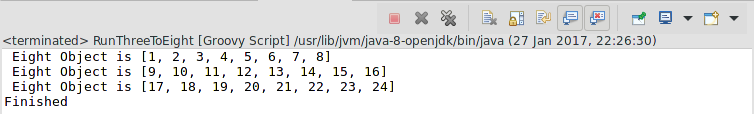
\includegraphics[width=\textwidth]{img/screenshots/2-2.png}


\subsubsection*{Questions}

\paragraph{1. What change is required to output objects containing six integers?}

To update the code to generate groups of 6 instead of 8 we can change the for loop in {\em CreateSetsOfEight.groovy} from \mintinline{groovy}{for ( int i in 0 .. 7 )} to \mintinline{groovy}{for ( int i in 0 .. 5 )}.

\paragraph{2. How could you parameterise this in the system to output objects that contain any number of integers (e.g. 2, 4, 8, 12) ?}

To parameterise the solution to any group size we can add a groupSize parameter to the output list generator.

\inputgroovy[label=CreateSetsParameterised.groovy,firstline=4]{../ChapterExercises/src/c2/CreateSetsParameterised.groovy}
\inputgroovy[label=RunThreeToAny.groovy,firstline=5]{../ChapterExercises/src/c2/RunThreeToAny.groovy}


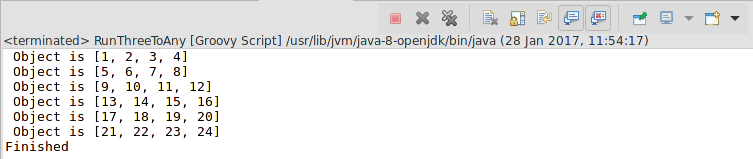
\includegraphics[width=\textwidth]{img/screenshots/2-2-q2.png}